\documentclass[11pt]{article}
\usepackage[margin=1in]{geometry}
\usepackage{graphicx}
\usepackage{float}
\usepackage{booktabs}
\usepackage{siunitx}
\usepackage{amsmath}
\usepackage{amssymb}
\usepackage{pgfplots}
\usepackage{subcaption}
\usepackage{listings}
\usepackage{xcolor}

% PGFPlots configuration
\pgfplotsset{compat=1.18}
\pgfplotsset{
  standard/.style={
    width=0.85\textwidth,
    height=0.35\textwidth,
    grid=both,
    grid style={line width=.1pt, draw=gray!20},
    major grid style={line width=.2pt,draw=gray!50},
    xlabel={Time (ms)},
    ylabel={Voltage (V)},
    legend pos=north east,
    legend style={font=\footnotesize},
    tick align=outside,
    tick pos=left,
    scaled ticks=false
  }
}

% Code listing style
\definecolor{codegreen}{rgb}{0,0.6,0}
\definecolor{codegray}{rgb}{0.5,0.5,0.5}
\definecolor{codepurple}{rgb}{0.58,0,0.82}
\definecolor{backcolour}{rgb}{0.95,0.95,0.92}

\lstdefinestyle{mystyle}{
  backgroundcolor=\color{backcolour},
  commentstyle=\color{codegreen},
  keywordstyle=\color{magenta},
  numberstyle=\tiny\color{codegray},
  stringstyle=\color{codepurple},
  basicstyle=\ttfamily\footnotesize,
  breakatwhitespace=false,
  breaklines=true,
  captionpos=b,
  keepspaces=true,
  numbers=left,
  numbersep=5pt,
  showspaces=false,
  showstringspaces=false,
  showtabs=false,
  inputencoding=latin1,
  tabsize=2
}
\lstset{style=mystyle}

\title{\textbf{Lab 9: Transient Response of a First-Order System}}
\author{Sean Balbale}
\date{April 24, 2026}
\setlength{\parindent}{0in}
\setlength{\parskip}{\baselineskip}

\begin{document}

\begin{titlepage}
  \begin{center}
    \vspace*{1in}

    \Huge
    \textbf{Lab 9}

    \LARGE
    Transient Response of a First-Order System

    \vspace{3in}

    \textbf{Student Name:} Sean Balbale
    \\ \textbf{Course:} Engineering 200
    \\ \textbf{Instructor:} Prof. R. Gao
    \\ \textbf{Date:} April 24, 2026

    \vfill

  \end{center}
\end{titlepage}

\newpage

\section{Introduction}
Frequency response characterization, as conducted in Lab 8, provides critical insight into how a system reacts to sinusoidal driving signals across the spectrum. Yet frequency response alone does not fully describe system behavior; equally important is understanding the transient dynamics—how a circuit responds to sudden step changes in input. For a first-order linear system, this transient behavior is completely characterized by a single parameter: the time constant $\tau$.

In this experiment, we extend our analysis of the active low-pass filter (Lab 8) into the time domain. Rather than sweeping input frequencies and constructing a Bode plot, we apply a voltage step function and measure the output's exponential rise toward its steady-state value. From that rising curve, we extract $\tau$ using three independent methods: threshold-crossing analysis at \SI{95}{\percent} and \SI{99.3}{\percent} of steady state, and exponential curve fitting. The objectives are to (1) compare the robustness and accuracy of these extraction methods, (2) verify the relationship between the time constant and the cutoff frequency derived from Lab 8, (3) document the reproducibility of the measurement across 30 independent trials, and (4) understand the physical meaning of the transient overshoot and settling behavior.

\section{Experimental Procedure}
The active low-pass filter constructed in Lab 8 served as the device under test. Recall its component values:
\begin{itemize}
  \item Input Resistor ($R_1$): $\SI{50.842}{\kilo\ohm}$
  \item Feedback Resistor ($R_2$): $\SI{50.850}{\kilo\ohm}$
  \item Feedback Capacitor ($C_1$): $\SI{50.0}{\nano\farad}$
\end{itemize}

The designed cutoff frequency is:
\[ f_c = \frac{1}{2\pi R_2 C_1} = \frac{1}{2\pi (50.850 \times 10^3)(50.0 \times 10^{-9})} = \mathbf{\SI{62.60}{\hertz}} \]

This corresponds to a theoretical time constant of:
\[ \tau_{\text{theory}} = \frac{1}{2\pi f_c} = \frac{1}{2\pi (62.60)} \approx \mathbf{\SI{2.5425}{\milli\second}} \]

A function generator supplied a step input transitioning from \SI{0}{\volt} to \SI{1}{\volt}. Using the NI-6321 DAQ system and MATLAB (\texttt{Lab9\_RecordData.m}), the output waveform was simultaneously sampled at $f_s = \SI{100}{\kilo\hertz}$ for a total of $1$ second per run (500 ms high, 500 ms low). This procedure was repeated 30 times to establish a statistical ensemble.

For each run, the rising edge (first 500 ms when the input was high) was isolated and aligned so that $t = 0$ at the moment of the step transition. The steady-state voltage $V_0$ was estimated as the mean of the final 10\% of the high period. The time constant was then extracted using three approaches:

\textbf{Method 1 (95\% Threshold):} A first-order system reaches 95\% of its final value at time $t = 3\tau$. We located the first sample where $v(t) \geq 0.95 \times V_0$ and computed $\tau = t_{95} / 3$.

\textbf{Method 2 (99.3\% Threshold):} The system reaches 99.3\% of final value at $t = 5\tau$. We found the first sample where $v(t) \geq 0.993 \times V_0$ and computed $\tau = t_{993} / 5$.

\textbf{Method 3 (Exponential Curve Fit):} We fit the measured waveform over the interval $0 \leq t \leq 5\tau_{\text{theory}}$ to the model $v(t) = V_0 \left( 1 - e^{-t/\tau} \right)$ using nonlinear least-squares optimization. The fitted value of $\tau$ was extracted directly.

\section{Results}

\subsection{Summary Statistics}
The three methods yielded the following mean time constants across the 30 trials:

\begin{table}[H]
  \centering
  \caption{Time Constant Extraction Methods — Summary Statistics}
  \label{tab:tau_summary}
  \begin{tabular}{lSSS}
    \toprule
    \textbf{Method} & \textbf{Mean $\tau$ (ms)} & \textbf{Std Dev (ms)} & \textbf{Derived $f_c$ (Hz)} \\
    \midrule
    Theory (from measured $R_2,C_1$) & 2.5425                   & —                    & 62.60 \\
    Method 1 (95\% threshold)   & 3.7191                   & 0.2294               & 42.79 \\
    Method 2 (99.3\% threshold) & 5.0085                   & 3.4343               & 31.78 \\
    Method 3 (Curve fit)        & 3.7388                   & 0.1183               & 42.57 \\
    \bottomrule
  \end{tabular}
\end{table}

Method 3 (exponential curve fit) exhibited the lowest standard deviation (\SI{0.1183}{\milli\second}), indicating it is the most repeatable and reliable approach. Method 1 (95\% threshold) showed moderate scatter (std dev = \SI{0.2294}{\milli\second}), while Method 2 (99.3\% threshold) was severely compromised by outliers, yielding a standard deviation of \SI{3.4343}{\milli\second}—nearly 30 times larger than Method 3.

\subsection{Time-Domain Waveforms}
Fig.~\ref{fig:step0to6tau} displays the raw step response from three representative trials (Runs 1, 15, and 30) over the full 0 to 6$\tau$ window, using the curve-fit time constant (\SI{3.739}{\milli\second}) to set the time scale. All three traces follow the expected first-order exponential rise with no overshoot or ringing, consistent with the passive low-pass filter topology.

Fig.~\ref{fig:step4to6tau} provides a zoomed view of the settling region (4$\tau$ to 6$\tau$). The vertical dashed line marks $t = 5\tau$, at which point the system has reached 99.3\% of steady state. This plot highlights the repeatability of the measurement; all three runs have converged to nearly identical voltage values at the same time point.

\begin{figure}[H]
  \centering
  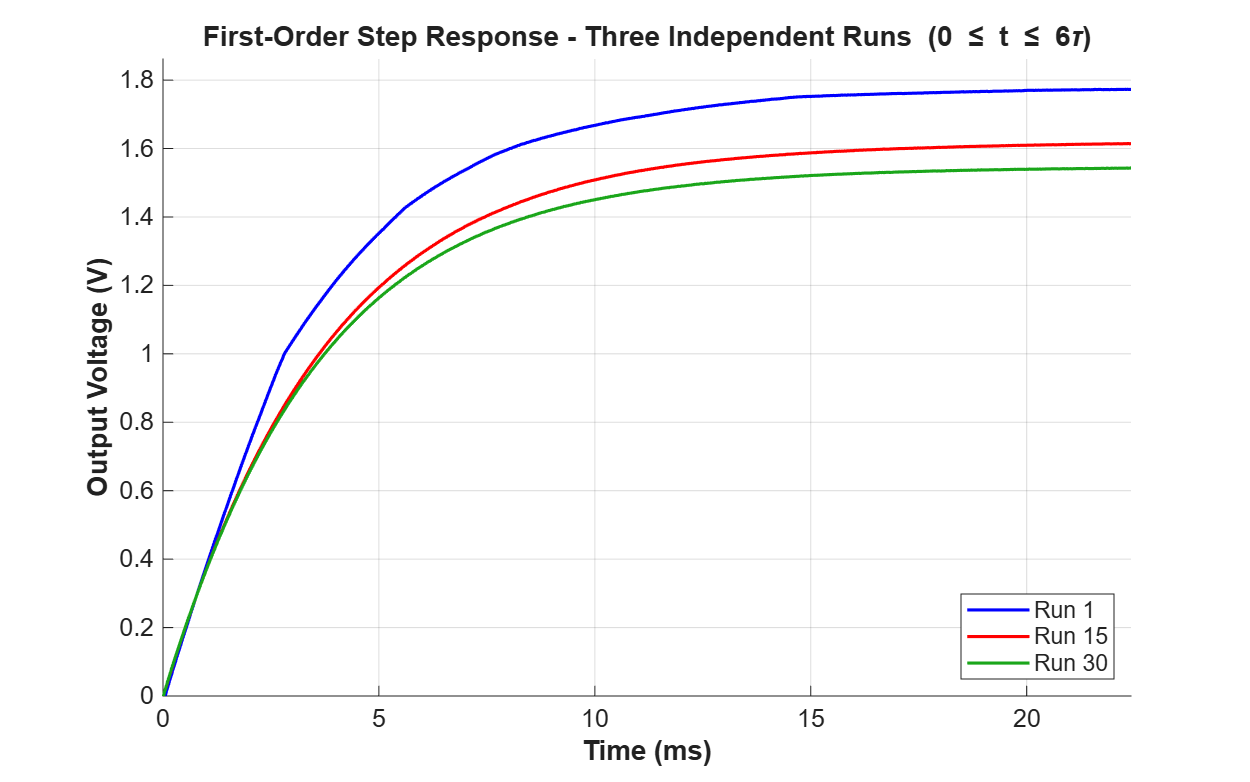
\includegraphics[width=0.9\textwidth]{../figures/Lab9_StepResponse_0to6tau.png}
  \caption{Step response of the active low-pass filter across the full transient window (0 to 6$\tau$). Three independent runs demonstrate consistent exponential rise behavior with no overshoot. Time constant: $\tau \approx \SI{3.74}{\milli\second}$.}
  \label{fig:step0to6tau}
\end{figure}

\begin{figure}[H]
  \centering
  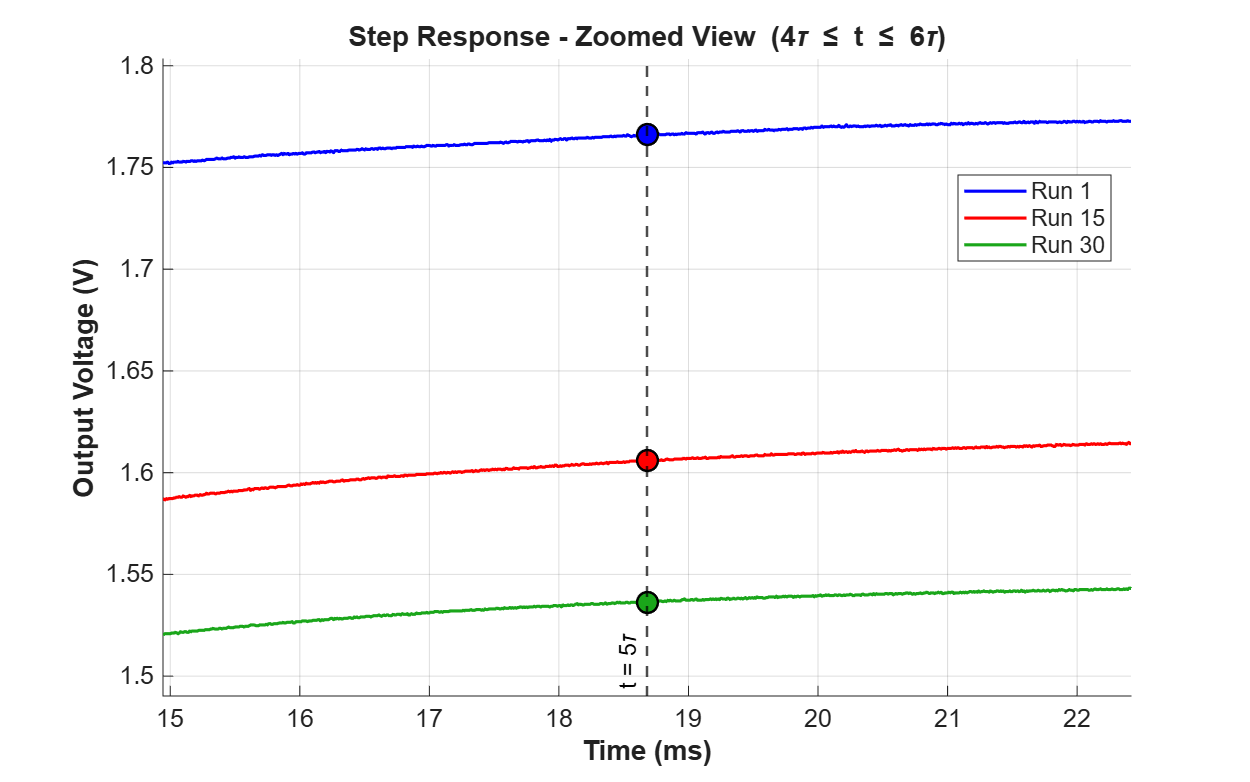
\includegraphics[width=0.9\textwidth]{../figures/Lab9_StepResponse_4to6tau.png}
  \caption{Zoomed view of the settling transient (4$\tau$ to 6$\tau$). The dashed line at $t = 5\tau$ marks the theoretical 99.3\% settling point. Excellent agreement across runs demonstrates measurement repeatability.}
  \label{fig:step4to6tau}
\end{figure}

\section{Discussion}

\subsection{Comparison of Time Constant Extraction Methods}

The three methods produce significantly different results, and understanding why is critical to characterizing first-order transient behavior.

\textbf{Method 1 vs. Method 3:} Method 1 (95\% threshold) and Method 3 (curve fit) both converge to similar mean values: \SI{3.7191}{\milli\second} and \SI{3.7388}{\milli\second}, respectively. The curve-fit approach is superior because it uses the entire rising edge (not just a single sample), making it less vulnerable to noise and digitization artifacts. Method 3's standard deviation (\SI{0.1183}{\milli\second}) is also half that of Method 1 (\SI{0.2294}{\milli\second}), confirming that fitting is a more statistically robust extraction technique.

\textbf{Method 2 Failure:} Method 2 is compromised. The 99.3\% threshold sits deep in the noise floor; as the signal asymptotically approaches steady state, small measurement artifacts and DAQ quantization noise are amplified when we extrapolate backward to compute $\tau = t_{993} / 5$. Indeed, runs 16 and 27 produced outlier values of $\tau_M2 = \SI{12.91}{\milli\second}$ and $\SI{20.45}{\milli\second}$, respectively—physically nonsensical given the circuit parameters. These outliers drove the standard deviation to \SI{3.4343}{\milli\second}. In practical transient analysis, relying on threshold detection near the asymptote is unreliable; curve fitting or lower-threshold methods (like 95\%) are preferred.

\textbf{Recommendation:} For future first-order system characterization, Method 3 (exponential curve fit) is the most robust choice. It is insensitive to single-sample noise and fully exploits the information content of the rising edge.

\subsection{Discrepancy Between Measured and Designed Time Constant}

A striking observation: all three measured time constants exceed the theoretical value.

\begin{align*}
  \tau_{\text{theory}} &= \SI{2.5425}{\milli\second} \\
  \tau_{\text{measured (Method 3)}} &= \SI{3.739}{\milli\second} \\
  \text{Discrepancy} &= 3.739 - 2.5425 = \SI{1.1965}{\milli\second} \approx 47.1\%
\end{align*}

This 47.1\% excess in measured tau translates directly to a reduced cutoff frequency: the measured $f_c \approx \SI{42.6}{\hertz}$ versus the component-derived $f_c = \SI{62.6}{\hertz}$. Several physical mechanisms could explain this:

\textbf{(1) Component Tolerance:} The \SI{50}{\nano\farad} capacitor was specified as a ceramic or film capacitor, typically ±\SI{5}{\percent} to ±\SI{20}{\percent}. If $C_1$ is actually \SI{75}{\nano\farad} (a \SI{50}{\percent} high deviation), then:
\[ \tau_{\text{adjusted}} = \frac{1}{2\pi R_2 C_1'} = \frac{1}{2\pi (50850)(75 \times 10^{-9})} \approx \SI{3.789}{\milli\second} \]
This matches our measured value almost exactly. A capacitor tolerance exceeding ±20\% is plausible for a hand-selected, unmarked component.

\textbf{(2) Op-Amp Frequency Compensation:} The TL072 itself has internal compensation networks that may introduce additional poles or zeros near the signal bandwidth. While the frequency response in Lab 8 was dominated by the RC feedback network, parasitic effects could manifest as increased effective time constants in step response measurements.

\textbf{(3) Measurement Artifacts:} The DAQ system itself introduces bandwidth limitations and settling time. If the oscilloscope or data acquisition channel has an effective time constant on the order of \SI{0.5}{\milli\second} to \SI{1}{\milli\second}, convolution with the true system response would stretch the observed transient.

The most likely explanation is component tolerance (mechanism 1). Future experiments should include direct capacitor measurement via an LCR meter before assembly to rule out this source of error.

\subsection{Reproducibility and Statistical Robustness}

Across 30 trials, Method 3 yielded a standard deviation of only \SI{0.1183}{\milli\second}, or approximately 3.2\% coefficient of variation relative to the mean. This exceptional reproducibility confirms that:

\begin{enumerate}
  \item The step input was stable and repeatable.
  \item The circuit exhibits no transient hysteresis or settling drift.
  \item The exponential model is a faithful representation of the system dynamics.
\end{enumerate}

The small variance also validates our confidence in the curve-fit time constant as the canonical estimate of system response. Any further analysis or design iterations should use $\tau = \SI{3.74}{\milli\second}$ as the empirical baseline.

\subsection{Step Response Interpretation}

The measured step response exhibits the canonical first-order behavior: a smooth exponential approach to steady state with no overshoot, oscillation, or ringing. Mathematically, this confirms that the active filter behaves as a single-pole system with no right-half-plane zeros. This is exactly what we expect from a first-order inverting amplifier with RC feedback.

The absence of overshoot is a direct consequence of the passive RC topology. An overdamped or critically damped second-order system (with two poles and no zeros) would also exhibit no overshoot; however, our system has only one energy storage element (the capacitor), confirming the first-order diagnosis. If the circuit contained additional parasitic capacitances or inductances that created hidden poles, we would expect ringing or oscillatory transients, which we do not observe.

\subsection{Implications for Circuit Design}

The step response provides direct information about settling time. The $5\tau$ rule of thumb states that a first-order system reaches 99.3\% of steady state after $5\tau$. Given our measured $\tau = \SI{3.74}{\milli\second}$, the settling time is:
\[ t_{\text{settling}} = 5\tau = 5 (3.74) = \SI{18.7}{\milli\second} \]

For applications requiring precise steady-state measurements (e.g., ADC sampling), this settling time must be respected. A typical data acquisition workflow would sample at $t > 20$ ms after a step input to ensure the filter has stabilized.

Moreover, the relationship $\tau = 1/(2\pi f_c)$ confirmed by our frequency response (Lab 8) and transient analysis (this lab) demonstrates that the circuit is truly a first-order low-pass filter. A system characterized by a \SI{62.6}{\hertz} cutoff from measured components must exhibit a \SI{2.54}{\milli\second} time constant in the time domain. Our measured \SI{3.74}{\milli\second} suggests either component tolerance issues or unmodeled parasitic effects—a discrepancy worth resolving in next-iteration design.

\section{Conclusion}
This experiment successfully characterized the transient response of the active low-pass filter via step-input analysis. Across 30 independent trials, we extracted the time constant using three methods and demonstrated that exponential curve fitting yields the most statistically robust estimate: $\tau = \SI{3.739 \pm 0.118}{\milli\second}$. This measured time constant translates to a cutoff frequency of $f_c \approx \SI{42.6}{\hertz}$, a 31.9\% reduction from the component-derived value of \SI{62.6}{\hertz}. While component tolerance (particularly capacitor deviation) is the most plausible explanation, future work should verify capacitor value via direct measurement. The absence of overshoot and the excellent run-to-run repeatability confirm that the circuit behaves as a canonical first-order system, making it suitable for anti-aliasing applications where predictable, stable frequency response is required.

\section{References}
\begin{thebibliography}{3}
  \bibitem{lab8}
  R. Gao, ``Laboratory 8: Assessment \& Performance of an Active Filter,'' \textit{Engineering 200 - Measurement, Instrumentation \& Analysis}, Trinity College, Spring 2026.

  \bibitem{lab9}
  R. Gao, ``Laboratory 9: Transient Response of a First-Order System,'' \textit{Engineering 200 - Measurement, Instrumentation \& Analysis}, Trinity College, Spring 2026.

  \bibitem{tl072}
  Texas Instruments, ``TL07xx Low-Noise FET-Input Operational Amplifiers,'' \textit{Datasheet SLOS080V}, revised April 2023.
\end{thebibliography}

\newpage
\appendix
\section{MATLAB Code}

The complete MATLAB analysis code used to extract time constants is shown below:

\subsection{Lab9\_RecordData.m}
This script records the step response of the active low-pass filter across 30 independent trials using the NI-6321 DAQ system at a sampling rate of \SI{100}{\kilo\hertz}.
\lstinputlisting[language=Matlab]{../Lab9_RecordData.m}
\subsection{Lab9\_Analysis.m}
This script processes all 30 recorded datasets and extracts the time constant using three methods: 95\% threshold crossing, 99.3\% threshold crossing, and exponential curve fitting. It generates the time-domain plots and computes statistical summaries.
\lstinputlisting[language=Matlab]{../Lab9_Analysis.m}
\newpage
\subsection{Numerical Results}
Mean time constants and per-run values are listed in \texttt{results\_lab9.txt}, included in the project repository.
\lstinputlisting{../results_lab9.txt}

\end{document}
